\documentclass{article}
\usepackage[utf8]{inputenc}
\usepackage{amsmath}
\usepackage{geometry}
\geometry{
 a4paper,
 total={182mm,257mm},
 left=14mm,
 top=20mm,
 }
 \usepackage[utf8]{inputenc}
 \usepackage[italian]{babel}
\usepackage[T1]{fontenc}
\usepackage{amssymb}
\usepackage{physics}
\usepackage{tikz}
\usepackage{graphicx}
\graphicspath{ {Immagini/Dinamica/} }
\usepackage{float}
\usepackage{hyperref}
\hypersetup{
    colorlinks=true,
    linkcolor=red,
    citecolor=green
    filecolor=magenta,      
    urlcolor=cyan,
}


%Theorem Environments
\newtheorem{thm}{Teorema}[section]
\newtheorem{lem}[thm]{Lemma}
\newtheorem{property}{Proprietà}[section]
\newtheorem{defn}{Definizione}[section]
\newtheorem{prop}[defn]{Proposizione}
\newtheorem{example}{Esempi}[subsection]
\newtheorem{exerc}[example]{Esercizi Svolti}

%Commandi di Formattazione
\newcommand{\noi}{\noindent}
\newcommand{\note}{\noindent {\quad \bf \underline{Osservazione:}} \quad}
\newcommand{\eg}{\noindent {\bf \underline{Esempio:}} \quad}
\newcommand{\bfemph}[1]{\textbf{\textit{#1}}}
\renewcommand{\emph}[1]{\bfemph{#1}}

%Number Sets
\newcommand{\R}{\mathbb{R}}
\newcommand{\C}{\mathbb{C}}
\newcommand{\Z}{\mathbb{Z}}
\newcommand{\Q}{\mathbb{Q}}

%Shortcuts
\newcommand{\then}{\ensuremath{\Rightarrow}}
\newcommand{\twopartdef}[4]
{
	\left\{
		\begin{array}{ll}
			#1 & \mbox{se } #2 \\
			#3 & \mbox{se } #4
		\end{array}
	\right.
}

%Vectors
\renewcommand{\i}{\vu{i}}
\renewcommand{\j}{\vu{j}}
\renewcommand{\k}{\vu{k}}
\renewcommand{\a}{\va{a}}
\renewcommand{\b}{\va{b}}
\renewcommand{\c}{\va{c}}
\renewcommand{\v}{\va{v}}
\renewcommand{\u}{\va{u}}
\newcommand{\s}{\va{s}}
\renewcommand{\t}{\va{t}}
\newcommand{\verst}{\vu{t}}
\newcommand{\versr}{\vu{r}}
\renewcommand{\r}{\va{r}}
\newcommand{\tauvs}{\vu{\tau}}
\newcommand{\tauvt}{\va{\tau}}
\newcommand{\normvs}{\vu{n}}
\newcommand{\N}{\va{N}}
\newcommand{\normvt}{\N}
\newcommand{\g}{\va{g}}
\newcommand{\F}{\va{F}}
\newcommand{\f}{\va{f}}
\newcommand{\p}{\va{p}}
\newcommand{\J}{\va{J}}




\title{Meccanica}
\author{Roberto Gargiulo}
\date{Today}

\begin{document}

\maketitle
\tableofcontents
\pagebreak


\section{Idee Fondamentali della Fisica}

\subsection{Grandezze Fisiche e la loro Misura}

\begin{defn}
Una \textbf{Grandezza Fisica} si definisce \textbf{operativamente} con una procedure di misurazione che associa ad essa un numero. \\
Si possono distinguere \textbf{Misure Empiriche}, associate ad uno strumento, e \textbf{Misure Assolute}, indipendenti dallo strumento. 
\end{defn}

\begin{defn}
La \textbf{Grandezza Misurata} di un fenomeno è una classe di equivalenza di cui si sceglie un \textbf{campione} che fornisce l'unità di misura della grandezza.
\end{defn}
\note Non è necessario stabilire campioni per ogni grandezza, in quanto grazie alle relazione matematiche tra le varie grandezze ci si può ricondurre ad un numero finito di grandezze "fondamentali". Un sistema formato da un certo numero di grandezze fondamentali è detto un \textbf{Sistema di Misura}.

Generalmente si fa uso del SI (Sistema Internazionale di Misura) che include 7 grandezze fondamentali:
\begin{center}
\begin{tabular}{ |c|c|c| }
\hline
Grandezza & Unità di Misura & Simbolo\\
\hline
Intervallo di Tempo & secondo & s\\
Lunghezza & metro & m\\
Massa & chilogrammo	& kg\\
Intensità di Corrente Elettrica	& ampere & A\\
Intensità Luminosa	& candela &	cd\\
Quantità di Sostanza & mole & mol\\
Temperatura Termodinamica &	kelvin & K\\
\hline
\end{tabular}
\end{center}

\subsubsection{Calcolo Dimensionale}
Il Calcolo Dimensionale si può riassumere in questi tre principi:
\begin{enumerate}
    \item La Somma tra Grandezze Equidimensionali produce una grandezza equidimensionale alle prime due
    \item Il Prodotto tra due Grandezze è produce una grandezze avente come dimensione il prodotto delle prime due. In particolare se le due grandezze hanno dimensioni elevate a una certa potenza in comune, la grandezza ha dimensioni uguali alla somma delle potenze delle dimensioni delle due grandezze.
    \item Gli argomenti delle funzioni devono essere adimensionali.
\end{enumerate}

\section{Geometria dei Vettori}

\begin{defn}
Un \textbf{Vettore} dello Spazio Geometrico è una classe di equipollenza formata da segmenti orientati.
\end{defn}

\begin{defn}
Il \textbf{Vettore Posizione} di un corpo che si trova nel punto P è un vettore geometrico applicato nell'origine del riferimento che collega l'origine al punto P. Esso è identificato (dato un riferimento) da una terna (coppia) di numeri reali.
\end{defn}

\begin{prop}
Nel Piano ha senso scegliere due possibili sistemi di riferimento:
\begin{enumerate}
    \item Un Sistema di Assi Cartesiani, che identifica un punto con la loro distanza (orientata) rispetto ai due assi (ortogonali, che si intersecano in un punto detto \textbf{origine}).
    \item Un Sistema Polare, formato da un punto detto \textbf{origine} è una semiretta avente come vertice tale punto detta \textbf{asse polare}, che identifica unicamente (ad eccezione dell'origine) un punto del piano tramite la distanza dall'origine e l'angolo formato tra l'asse polare e la semiretta originatasi nell'origine e passante per il punto.
\end{enumerate}
\end{prop}
\begin{property}
\hypertarget{formulecoordinate}{
Le \textbf{Formule di Cambiamento di Coordinate} tra un Sistema Cartesiano e uno di coordinate polari sono date dai sistemi}:
\[\left\{
		\begin{array}{l}
			x=r\cos\Phi  \\
			y=r\sin\Phi  \\
		\end{array}
	\right.\iff
	\left\{
		\begin{array}{l}
			r=\sqrt{x^2+y^2}  \\
			\Phi=\arctan\left(\frac{y}{x}\right)\,\vee\,\pm\frac{\pi}{2}  \\
		\end{array}
	\right.\]
\end{property}

\begin{property}
La \textbf{Traslazione} è un'isometria definita dal seguente sistema:
\[\left\{
		\begin{array}{l}
			x'=x+u_x  \\
			y'=y+u_y  \\
		\end{array}
	\right.\quad\text{dove}\, \va{u}=(u_x,u_y)\,\text{è il vettore di traslazione}\]
\end{property}

\begin{property}
La \textbf{Rotazione} centrata nell'origine è una trasformazione definita dalla seguente matrice ortogonale (sistema associato):
\[\begin{pmatrix}\cos\theta&-\sin\theta\\\sin\theta&\cos\theta\\\end{pmatrix}\iff\left\{
\begin{array}{l}
    x'=\cos\theta-y\sin\theta   \\
    y'=x\sin\theta+y\cos\theta   \\
\end{array}\right.\]
\end{property}

\note Il Vettore Posizione ha modulo invariante rispetto alle rotazioni centrate nell'origine ma cambia nelle traslazioni.
\note I Vettori non applicati nell'origine hanno moduli invarianti sia nelle rotazioni che nelle traslazioni. Tale è il caso del \textbf{Vettore Spostamento}.

\begin{defn}
Il \textbf{Vettore Spostamento} è il vettore dato dalla differenza tra due vettori posizione.
\end{defn}

\subsection{Operazioni tra Vettori}

\begin{defn}
L'\textbf{addizione} tra vettori geometrici è data dal metodo punta-coda (oppure equivalentemente il metodo del parallelogramma):
\[
\begin{tikzpicture}
\draw[->,thick](0,0) -- (2,3);
\draw[->,thick](2,3) -- (5,1);
\draw[->,thick,blue](0,0) -- (5,1);
\end{tikzpicture}
\]
Oppure in componenti:
\[\va{a}+\va{b}=(a_x+b_x,a_y+b_y,a_z+b_z)\]
Notiamo che essa è commutativa e associativa.
\end{defn}

\begin{defn}
Il \textbf{prodotto esterno} tra vettore e scalare conserva la sua direzione, ed è tale che il modulo del vettore così ottenuto è uguale al modulo del vettore iniziale moltiplicato per il valore assoluto dello scalare. Si può definire in componenti come segue:
\[m\va{a}=(ma_x,ma_y,ma_z)\]
Anche tale operazione è commutativa e associativa e inoltre gode della proprietà distributiva rispetto all'addizione.
\end{defn}

\begin{defn}
Un \textbf{versore} è un vettore di modulo 1.
\end{defn}
\note Il vettore \(\vu{a}=\frac{\va{a}}{|\va{a}|}\) è un versore.

\begin{defn}
Il \textbf{Prodotto Scalare} si definisce come segue:
\[\va{a}\vdot\va(b)=|a||b|\cos\theta\]
Oppure in componenti:
\[\va{a}\vdot\va{b}=a_xb_x+a_yb_y+a_zb_z\]
In quanto:
\[\begin{array}{l}
    \vu{i}\vdot\vu{i}=0\\
    \vu{j}\vdot\vu{j}=0\\
    \vu{k}\vdot\vu{k}=0\\
\end{array}\quad\va{a}\vdot\va{b}=(a_x\i+a_y\j+a_z\k)\vdot(b_x\i+b_y\j+b_z\k)\]
Il prodotto scalare è commutativo e distributivo rispetto alla somma.
\end{defn}
\begin{property}
Il Prodotto Scalare è invariante rispetto alle rotazioni centrate nell'origine.
\end{property}

\begin{defn}
\textbf{Componente Ortogonale} di un vettore $\b$ lungo un altro vettore $\b$ è il numero $\b_a=\b\vdot\vu{a}$
\end{defn}

\begin{thm}[Teorema di Carnot]
Dati \(\a,\b,\c\) tali che \(\a+\b=\c\) allora risulta 
\[|\c|^2=|\a^2|+|\b|^2+|\a||\b|\cos\theta\]
\end{thm}

\begin{defn}
Il \textbf{Prodotto Vettoriale} è un'operazione tra vettori tridimensionali che restituisce un vettore tale che:
\begin{enumerate}
    \item Verso e Direzione di $\a\times\b$ sono individuati dalla regola della mano destra.
    \item \(|\a\times\b|=|\a||\b|\sin\theta\)
\end{enumerate}
Geometricamente, immaginando i vettori $\a,\b$ come spostamenti, allora $|\a\times\b|$ è l'area del parallelogramma che ha per lati $|\a|,|\b|$ (infatti le sue altezze sono $|\a|\sin\theta,|\b|\sin\theta$.
Il Prodotto Scalare gode delle seguenti proprietà:
\begin{enumerate}
    \item Il prodotto vettoriale di vettori paralleli è il vettore nullo e in particolare $\i\times\i=\j\times\j=\k\times\k=\va{0}$.
    \item Il prodotto vettoriale è anticommutativo.
    \item Il prodotto vettoriale gode della proprietà distributiva rispetto all'addizione.
\end{enumerate}


Come regola di calcolo, note le componenti dei vettori, è possibile calcolare il prodotto vettoriale come il determinante della seguente matrice:
\[\begin{vmatrix}\i&\j&\k\\ a_x&a_y&a_z\\b_x&b_y&b_z\\ \end{vmatrix}=(a_yb_z-a_zb_y)\i+(a_zb_x-a_xb_z)\j+(a_xb_y-a_yb_x)\k\]
\end{defn}

\begin{defn}
Il \textbf{Triplo Prodotto Scalare} di tre vettori non nulli è il numero $(\a\times\b)\vdot\c$ tale che $|(\a\times\b)\vdot\c|$ è il volume del parallelepipedo che ha per dimensioni i tre vettori. Si verifica che scambiando ciclicamente i tre vettori, il prodotto non cambia:
\[(\a\times\b)\vdot\c=(\c\times\a)\vdot\b=(\b\times\c)\vdot\a\]
Mentre uno scambio non ciclico fa cambiare di segno.
Si dimostra che:
\[(\a\times\b)\vdot\c=\begin{vmatrix}c_x&c_y&c_z\\ a_x&a_y&a_z\\b_x&b_y&b_z\\ \end{vmatrix}\]
\end{defn}

\begin{defn}
Il \textbf{Triplo Prodotto Vettoriale} è il vettore $(\a\times\b)\times\c$ che gode delle seguenti identità:
\[(\a\times\b)\times\c=(\a\vdot\c)\vdot\b-(\b\vdot\c)\vdot\a\]
\[\a\times(\b\times\c)=(\a\vdot\c)\vdot\b-(\a\vdot\b)\vdot\c\]
\end{defn}

\section{Cinematica del Corpo Puntiforme}


\subsection{Prime Definizioni}
\begin{defn}
La \textbf{Cinematica} consiste nella descrizione del Moto di un Corpo/Sistema di Corpi.
\end{defn}
\begin{defn}
Lo \textbf{Stato di Moto} è uno stato in cui il corpo cambia la propria posizione nel tempo.
\end{defn}

\begin{defn}
Si definisce \textbf{Punto Materiale} un qualunque corpo le cui dimensioni sono trascurabili rispetto allo spazio in cui può muoversi oppure rispetto ai corpi con cui può reagire.
\end{defn}

\begin{defn}
La \textbf{Traiettoria} si definisce come la curva continua che collega tutte le posizioni successive di un corpo in movimento.
\end{defn}

\subsection{I Moti Rettilinei}

\begin{defn}
\textbf{Velocità Media} \(v_m=\frac{x-x_0}{t-t_0}\)
\end{defn}
\begin{defn}
\textbf{Velocità Istantanea} \(v(t)=\dv{x(t)}{t}\)
\end{defn}
\note \(v_m=\frac{1}{t-t_0}\int_{t_0}^tv(t)dt\)
\begin{defn}
\textbf{Accelerazione Media} \(a_m=\frac{v-v_0}{t-t_0}\)
\end{defn}
\begin{defn}
\textbf{Accelerazione Istantanea} \(a(t)=\dv{v(t)}{t}=\dv[2]{x(t)}{t}\)
\end{defn}
\note \(a_m=\frac{1}{t-t_0}\int_{t_0}^ta(t)dt\)

\begin{defn}
\textbf{Moto Rettilineo Uniforme} Un moto rappresentato dall'equazione (scelto un opportuno riferimento in cui un'asse coincide con la retta su cui si muove il corpo):
\[x(t)=B(t-t_0)+A\]
Dove:
\begin{enumerate}
    \item B è la velocità iniziale $v_0$
    \item A è la posizione iniziale $x_0$
    \item t è l'istante (compreso tra quello iniziale e finale) in cui consideriamo il corpo.
    \item $t_0$ è l'istante in cui il corpo inizia a muoversi di moto rettilineo uniforme.
\end{enumerate}
La velocità è data dalla derivata \(\dv{x(t)}{t}=v(t)=v_0\) e risulta costante.
\end{defn}
\begin{defn}
\textbf{Moto Rettilineo Smorzato Esponenzialmente} Un moto la cui legge oraria è soluzione della seguente equazione differenziale:
\[\dv{v(t)}{t}=-kv\quad v(t_0)=v_0, k>0\]
Che si riconduce al moto rettilineo uniforme nel caso $k=0$. Ha soluzione generale:
\[v(t)=v_0e^{-kt}\then x(t)=x_0+\int_{t_0}^tv(t)dt=\frac{v_0}{k}(1-e^{-kt})\]
Inoltre si definisce $\tau=\frac{1}{k}$ \textbf{costante di tempo}, tale che il rapporto tra la velocità iniziale e quella dopo un certo intervallo di tempo $\tau$ ha valore $e^{-1}$.
\end{defn}

\begin{defn}
\textbf{Moto Uniformemente Accelerato} Un moto descritto da un'equazione del tipo:
\[x(t)=x_0+v_0(t-t_0)+\frac{1}{2}a_0(t-t_0)^2\]
Che ha velocita $v(t)=\dv{x(t)}{t}=v_0+a_0(t-t_0)$ e accelerazione $a(t)=\dv{v(t)}{t}=a_0$ costante.
Se l'accelerazione iniziale è positiva allora il grafico posizione-tempo è una parabola convessa (viceversa se è negativa allora il grafico è una parabola concava).
\end{defn}
\note Un particolare tipo di moto uniformemente accelerato è il moto di caduta libera (con posizione e velocità iniziali):
\[x(t)=x_0+v_0(t-t_0)-\frac{1}{2}g(t-t_0)^2\quad v(t)=v_0-g(t-t_0)\quad a(t)=-g=-9,8 m/s^2\]
\begin{property}
\hypertarget{formulemotounifacc}{Possiamo stabilire formule per posizioni/velocità notevoli in un Moto di caduta libera}:
\begin{enumerate}
    \item Se la velocità iniziale è ha verso opposto a quello dell'accelerazione, allora raggiunge la massima altezza quando la velocità si annulla:
    \[v(\overline{t})=v_0+g(\overline{t}-t_0)=0\iff \overline{t}=t_0+\frac{v_0}{g}\]
    \item Il tempo di volo (caduta) è il tempo trascorso tra l'istante iniziale è l'istante in cui il corpo giunge al suolo, ossia quando la posizione è "nulla":
    \[x(t)=x_0+v_0(t-t_0)-\frac{1}{2}g(t-t_0)^2=0\iff t=\frac{gt_0+v_0\pm\sqrt{v_0^2+2gx_0}}{g}\quad v(t)=\pm\sqrt{v_0^2+2gx_0}\]
\end{enumerate}
\end{property}

\begin{defn}
\hypertarget{armonicosemplice}{
\textbf{Moto Armonico Semplice} Un moto avente per legge oraria}:
\[x(t)=A\sin(\omega t+\phi)\]
Dove:
\begin{enumerate}
    \item A è l'\textbf{ampiezza del moto}
    \item $\omega$ è la \textbf{pulsazione} (o velocità angolare)
    \item $\phi$ è la \textbf{fase iniziale}
\end{enumerate}
Inoltre si definiscono:
\begin{enumerate}
    \item \textbf{Periodo} $T=\frac{2\phi}{\omega}$
    \item \textbf{Frequenza} $\nu=\frac{1}{T}$
\end{enumerate}
Mentre velocità e accelerazione:
\[v(t)=A\omega\cos(\omega t+\phi)=\omega x(t)\]
\[a(t)=-A\omega^2\sin(\omega t+\phi)=-\omega^2 x(t)\]
La \textbf{condizione sufficiente} per cui un moto sia armonico è data dall'equazione differenziale:
\[\dv[2]{x(t)}{t}+\omega^2x(t)=0\]
\end{defn}


\begin{prop}
\hypertarget{accelerazioneinascissa}{In numerose situazioni in cui è nota la traiettoria e quindi $x(t)$ nella sua completezza, risulta utile considerare velocità e accelerazione in funzione della posizione invece che del tempo.} Notiamo che:
\[a=\dv{v[x(t)]}{t}=\dv{v(x)}{x}\dv{x}{t}=\dv{v(x)}{x}v\then \int adx=\int vdv \iff \int_{x_0}^xadx=\int_{v_0}^v{vdv}=\eval{\frac{v^2}{2}}_{v_0}^v=\frac{v^2-v_0^2}{2}\]
Consideriamo i moduli di velocità/accelerazione nei moti notevoli appena discussi:
\begin{enumerate}
    \item Moto Uniformemente Accelerato:
    \[\int_{x_0}^xadx=a(x-x_0)\then v^2(x)=v_0^2+2a(x-x_0)\]
    Ciò indice che se il corpo non parte dal punto in cui la velocità si annulla, allora non esiste una sola funzione capace di descrivere l'intero moto (ossia la funzione non è strettamente monotona su tutto il suo dominio, quindi non è invertibile su un intervallo)
    \item Moto Armonico Semplice:
    \[\int_{x_0}^xadx=-\omega^2\int_{x_0}^xxdx=\frac{1}{2}\omega^2(x_0^2-x^2)\then v^2(x)=v_0^2+\omega(x_0^2-x^2)\]
    \item Moto Rettilineo Smorzato Esponenzialmente:
    \[a=-kv,\,adx=vdv\then -kvdx=vdv\iff -kdx=dv\iff -k(x-x_0)=v-v_0\then v=v_0-k(x-x_0) \]
\end{enumerate}
\end{prop}

\subsection{I Moti Piani}

In un moto piano risulta necessario parlare non solo di posizione, velocità e accelerazione come scalari ma come vettori.
Fissato un sistema di assi cartesiani (oppure un sistema di coordinate polari) ha senso quindi parlare di vettore posizione o \textbf{raggio vettore}:
\[\r(t)=\begin{pmatrix}x(t)\\y(t)\\\end{pmatrix}\iff \r(t)=\begin{pmatrix}r(t)\\\theta\\\end{pmatrix}\]
Usando le già note \hyperlink{formulecoordinate}{Formule di Cambiamento delle Coordinate}. Dobbiamo quindi generalizzare la definizione di velocità e accelerazione come vettori.

\begin{defn}
\textbf{Vettore Spostamento} \(\Delta\r=\r(t+\Delta t)-\r(t)\)
\end{defn}

\begin{prop}
La \textbf{Derivata di una Funzione Vettoriale} (dipendente da uno scalare) \(\v(t)=\dv{\r(t)}{t}\)
Questo vettore geometricamente è il vettore tangente alla traiettoria del punto in un certo istante t, infatti:
\[\a(t)\vdot\a(t)=0\iff \dv{\a\vdot\a}{t}=0\iff \dv{\a}{t}\a+\a\dv{\a}{t}=0\iff 2\a\dv{\a}{t}=0\iff \a\vdot\dv{\a}{t}=0\iff \a\perp\dv{\a}{t}\]
In particolare, fissato un sistema di riferimento cartesiano:
\[\r(t)=\begin{pmatrix}x(t)\\y(t)\\\end{pmatrix}\then\v(t)=\begin{pmatrix}x'(t)\\y'(t)\\\end{pmatrix}\]
Risulta talvolta utile separare l'analisi del cambiamento del modulo della velocità e della sua direzione e verso, a tale scopo utilizziamo il versore tangente \(\u_T(t)=\frac{\v(t)}{|\v(t)|}=\frac{\v(t)}{v(t)}\) tale che \(\v(t)=v(t)\u_T(t)=\dv{s(t)}{t}\u_T(t)\)

Notiamo infine che siccome la derivata di un vettore dipende dal vettore spostamento, allora anche essa non dipende dal cambiamento di riferimento.
\end{prop}

\begin{prop}
La \textbf{traiettoria} di un corpo che si muove in un piano può essere descritta da una certa equazione del tipo:
\[F(x,y)=0\]
Inoltre, se $\dv{F(x,y)}{y}\neq0,\dv{F(x,y)}{x}\neq0$ allora $x=x(t),y=y(t)$ sono funzioni invertibili, permettendo quindi di isolare $t$ in una delle due equazioni e sostituirla nell'altra, ottenendo un'equazione del tipo $F(x,y)=0$.
\end{prop}

\begin{defn}
\textbf{Velocità Vettoriale Media} $\va{v}_m=\frac{\Delta\r}{\Delta t}$
\end{defn}

\begin{defn}
\textbf{Velocità Vettoriale Istantanea} $\va{v}=\dv{r}{t}=\lim\limits_{\Delta t\to 0}\frac{\Delta\r}{\Delta t}$
\end{defn}

\begin{prop}[Velocità Tangenziale e Radiale]
Nel trattare la derivata di un vettore, specialmente nel caso si tratti del vettore posizione, risulta particolarmente utile usare un sistema di coordinate polari.\\

Detto $\u_r$ il versore della direzione di $\r$ e $\u_\theta$ il versore ortogonale ad essa istante per istante (cioè il vettore ottenuto ruotando $\u_r$ di $\frac{\pi}{1}$). Allora fissato un sistema di coordinate cartesiane (e uno di coordinate polari corrispondente) risulta:
\[\u_\theta(t)=\begin{pmatrix}0&-1\\1&0\\\end{pmatrix}\begin{pmatrix}\cos\theta\\\sin\theta\end{pmatrix}=\begin{pmatrix}-\sin\theta\\\cos\theta\\\end{pmatrix}\]

\[\r(t)=r\u_r(t)\then \v(t)=\dv{r\u_r(t)}{t}=\dv{r}{t}\u_r(t)+r\dv{\u_r(t)}{t}=\dv{r}{t}\u_r(t)+r\dv{[\cos[\theta(t)]\i+\sin[\theta(t)]\j]}{t}=\]\[=\dv{r}{t}\u_r(t)+\left[-r\theta'(t)\sin\theta\i+\theta'(t)\cos\theta\j\right]=\dv{r}{t}\u_r(t)+\theta'(t)[\sin\theta\i+\cos\theta\j]=\dv{r}{t}\u_r(t)+\theta'(t)\u_\theta(t)=\v_r+\v_\theta\]\\
\linebreak
Definiamo $\v_r$ la \textbf{velocità radiale} che ha modulo $\dv{r}{t}$ e direzione parallela ad $\r$; mentre $\v_\theta$ è la \textbf{velocità} trasversa o \textbf{tangenziale}, ortogonale ad $\r$ e di modulo $r\dv{\theta}{t}=r\omega$.
Usando come riferimento quello formato dai vettori $\u_r,\u_\theta$ allora il modulo della velocità vale:
\[v=\sqrt{\left(\dv{r}{t}\right)^2+\left(r\dv{\theta}{t}\right)^2}\]
\end{prop}


\begin{prop}
Nota la posizione (velocità) iniziale, si può passare da velocità (accelerazione) a posizione (velocità) usando l'integrale:
\[\r(t)=\r(t_0)+\int_{t_0}^t\v(t)dt\]
Dove:
\[\int_{t_0}^t\v(t)dt=\begin{pmatrix}\int_{t_0}^tx'(t)\\ \\ \int_{t_0}^ty'(t)\end{pmatrix}\]
\end{prop}

\begin{defn}
\textbf{Accelerazione Vettoriale Istantanea} \(\a(t)=\dv{\v}{t}=\dv[2]{\r}{t}\)
\end{defn}

\begin{prop}[Accelerazione Tangenziale e Centripeta]
Come per la velocità, possiamo esprimere l'accelerazione in termini di versori perpendicolari tra loro: il \textbf{versore tangenziale} $\u_T$ (che indica la direzione e il verso della velocità) e il \textbf{versore normale} $\u_N$ (ossia l'equivalente del versore $\u_\theta$ della velocità, scelto in modo che punti nel verso in cui punta la concavità della curva in ogni punto). Otteniamo quindi:
\[\a(t)=\dv{(v\u_T)}{t}=\dv{v}{t}\u_T+v\dv{\u_T}{t}=\dv{v}{t}\u_T+v\dv{\phi}{t}\u_N\]\\
Dove $d\phi$ è l'angolo tra i vettori $\u_T(t)$ e $\u_T(t+\delta t)$. Inoltre le rette normali alla traiettoria negli istanti $t$ e $t+\delta t$ si incontrano in punto detto \textbf{centro di curvatura}, ossia il centro della circonferenza tangente la curva della traiettoria in un intorno di $t$ (tale circonferenza è detta \textbf{osculatrice} ed è la circonferenza che meglio approssima la traiettoria).\\
\hypertarget{velangolare}{Possiamo poi esplicitare il valore di $\dv{\phi}{t}$ notando che dato l'arco infinitesimo $\dd s$ esso è uguale a $R\dd \phi$ dove R è il raggio della circonferenza osculatrice ed è detto} \textbf{raggio di curvatura}.\\
Risulta quindi:
\[\dv{\phi}{t}=\dv{\phi}{s}\dv{s}{t}=\frac{1}{R}v\]
E infine:
\[\a(t)=\dv{v}{t}\u_T+\frac{v^2}{R}\u_N=\a_T+\a_N\]
Chiamiamo $\a_T=\dv{v}{t}\u_T$ l'accelerazione \textbf{tangenziale} (dove $|\a_T|=a_s(t)$ e $\a_N$ l'accelerazione \textbf{centripeta} in quanto rivolta sempre verso il centro di curvatura.\\
\linebreak
Queste due componenti ci permettono poi di individuare moti già studiati:
\begin{enumerate}
    \item Quando $\a_N$ si annulla allora il moto è rettilineo (ossia la direzione della velocità non cambia).
    \item Quando $\a_T$ si annulla allora il moto è uniforme (ossia il modulo della velocità non cambia).
    \item Se sono entrambe nulle allora il moto è rettilineo uniforme.
\end{enumerate}
Inoltre il modulo dell'accelerazione risulta uguale a:
\[|\a(t)|=\sqrt{\left(\dv{v}{t}\right)^2+\frac{v^4}{R^2}}\]
\end{prop}
\note Nello spazio si sceglie il vettore \textbf{binormale} $\b=\tauvs\times\normvs$.

\subsection{Moto Circolare}

\begin{prop}[Ascissa Curvilinea]
\hypertarget{ascissacurv}{
In alcune situazioni risulta particolarmente utile (fissato un certo punto e un verso di percorrenza della curva) considerare la lunghezza di un arco il cui secondo punto è variabile lungo la curva.\\
Data la curva descritta da $\gamma(t)$ in un riferimento cartesiano tale che}:
\[\gamma(t)=\begin{pmatrix}x(t)\\y(t)\\\end{pmatrix}\] 
Più precisamente possiamo definire l'\textbf{ascissa curvilinea}:
\[s(t)=\int_{t_0}^t|\gamma'(u)|du=\int_{t_0}^t \sqrt{x'^2(u)+y'^2(u)}du\]
Da cui ricaviamo i moduli della velocità e dell'accelerazione tangenziale:
\[|\v(t)|=v_s(t)=\dv{s(t)}{t}=\sqrt{x'^2(t)+y'^2(t)}\]
\[|\a_T(t)|=a_s(t)=\dv{v(t)}{t}\]
Con l'uso dell'ascissa curvilinea siamo quindi capaci di ridurre un problema bidimensionale ad uno unidimensionale. Particolarmente utile è questa scelta nello studio dei moti circolari.
\end{prop}


\begin{defn}
Un \textbf{Moto Circolare} è un moto piano in cui l'accelerazione centripeta è costante e non nulla.
In particolare il \textbf{Moto Circolare Uniforme} è un moto in cui l'accelerazione tangenziale è nulla, mentre il \textbf{Moto Circolare Uniformemente Accelerato} è un moto in cui l'accelerazione tangenziale è costante (non nulla).
\end{defn}
\begin{property}[Proprietà del Moto Circolare]
Fissato un riferimento cartesiano nel centro della circonferenza e considerato l'angolo $\phi$ tra il raggio vettore e l'asse $x$ possiamo definire velocità e accelerazione angolare:
\begin{enumerate}
    \item Velocità Angolare $\omega=\dv{\phi}{t}$
    \item Accelerazione Angolare $\alpha=\dv{\omega}{t}=\dv[2]{\phi}{t}$
\end{enumerate}
Ricordando le considerazioni fatte nello studio dell'\hyperlink{velangolare}{accelerazione vettoriale} risulta:
\[\omega=\frac{v_s}{R}\quad\alpha=\frac{1}{R}\dv{v_s}{t}=\frac{a_s}{R}\]
E in particolare possiamo facilmente passare da ascissa curvilinea, velocità e accelerazione tangenziale ad angolo, velocità angolare ed accelerazione angolare moltiplicando (dividendo) per $R$:
\[s(t)=R\phi(t)\quad v_s(t)=R\omega(t)\quad a_s(t)=R\alpha(t)\]
Il moto circolare è inoltre un moto periodico, come si può notare esplicitando le componenti del raggio vettore a ogni istante:
\[\r(t)=\begin{pmatrix}x(t)\\y(t)\end{pmatrix}=\begin{pmatrix}R\cos(\omega t+\phi_0)\\R\sin(\omega t+\phi_0)\end{pmatrix}\]
Si può ottenere inoltre la legge oraria angolare e la legge oraria della velocità usando l'integrale, secondo quanto già visto.
La legge oraria angolare del moto circolare uniforme risulta infine:
\[\alpha(t)=0\then \phi(t)=\phi_0+\omega_0(t-t_0)\]
Mentre quella del moto circolare uniformemente accelerato (nella componente tangenziale):
\[\alpha(t)=\alpha_0\then\phi(t)=\phi_0'+\omega_0(t-t_0)+\frac{1}{2}\alpha (t-t_0)^2\]
Queste leggi però non descrivono completamente il moto, in quanto mancano dell'informazione riguardo l'accelerazione centripeta, che però può essere calcolata nota la velocità angolare, secondo la relazione già discusse (in quanto direzione e verso sono rispettivamente parallela e opposto a quelli del raggio vettore):
\[\a_N(t)=\frac{v^2}{R}\u_N=R\omega^2\u_N\]
\end{property}

\begin{prop}[Accelerazione in Funzione dell'Angolo]
Il moto circolare uniformemente circolare si può ricondurre (studiandone solo il comportamento tangenziale) a un moto uniformemente circolare e \hyperlink{accelerazioneinascissa}{similmente} possiamo ricondurre l'accelerazione angolare direttamente all'angolo, tale che:
\[\int_{\phi_0}^\phi \alpha(\theta)\dd \theta=\frac{\omega^2-\omega_0^2}{2}\]
\end{prop}

\begin{prop}[Rappresentazione Intrinseca]
Siccome risulta possibile considerare la legge oraria di un corpo in moto circolare tramite l'ascissa curvilinea, possiamo definire una rapprentazione \textbf{intrinseca}:
\[\left\{\begin{array}{l}
    \r(s(t))  \\
    s(t)  \\
\end{array}\right.\]
Che include la parametrizzazione della curva della traiettoria in funzione dell'ascissa curvilinea (cosa possibile in quanto per definizione di ascissa curvilinea $|\r'(t)|>0$ e quindi è crescente, quindi invertibile) e la funzione dell'ascissa curvilinea stessa, da cui si possono derivare velocità e accelerazione del corpo.
\end{prop}

\subsubsection{Moto Circolare tramite i Vettori Ruotanti}
Per comodità è possibile anche evitare lo studio  dei vettori bidimensionali e delle loro derivate nel caso generale e limitarsi solo al caso specifico dei \textbf{Vettori Ruotanti}, che permettono un intuitiva spiegazione del Moto Circolare e immediata derivazione delle leggi oraria di velocità e accelerazione come vettori.

\begin{defn}
Un \textbf{Vettore Ruotante} è un qualunque vettore bidimensionale di modulo costante che varia di verso e direzione e si può trasportare parallelamente a un certo punto O, in cui fissiamo il centro del nostro riferimento. Siccome è particolarmente importante lo studio di tale vettore per il Moto Circolare, studieremo più in particolare il suo comportamento (e in particolare la sua derivata) per dedurre velocità e accelerazione di un corpo il cui raggio vettore è un vettore ruotante.
\end{defn}


\begin{prop}[Derivata di un Vettore Ruotante]
\hypertarget{vettruotante}{Dato un vettore ruotante $\va{A}$ rispetto alla variabile $t$ (considerando per comodità solo la rotazione in senso antiorario, in modo che la variazione dell'angolo tra due vettori successivi sia positiva - $\Delta\phi>0$), consideriamo i versori $\normvs$ e $\normvs'$ uno perpendicolare alla direzione di $\Delta \va{A}$ e l'altro parallelo, in modo che puntino sempre dalla parte antioraria indipendentemente dal senso della rotazione.}
Consideriamo quindi il rapporto incrementale, notando che il triangolo formato dai vettori $\va{A(t)},\va{A(t+\Delta t)},\delta\va{A}$ è isoscele in quanto il modulo del vettore ruotante non cambia, pertanto $|\Delta\va{A}|=|\va{A(t)}|2\sin{\frac{\Delta\phi}{2}}$:
\[\frac{\Delta \va{A}}{\Delta t}=\frac{|\Delta\va{A}|\normvs'}{\Delta t}=|\va{A}|\frac{\Delta\phi}{\Delta t}\frac{\sin{\frac{\Delta\phi}{2}}}{\frac{\Delta\phi}{2}}\normvs'\]
Calcolando il limite per $\Delta t\to 0$ otteniamo quindi la derivata del vettore rispetto a t, notando che $\normvs'\to\normvs$ per $\Delta t\to 0$:
\[\lim_{\Delta t\to 0}\frac{\Delta \va{A}}{\Delta t}=\lim_{\Delta t\to 0} |\va{A}|\frac{\Delta\phi}{\Delta t}\frac{\sin{\frac{\Delta\phi}{2}}}{\frac{\Delta\phi}{2}}\normvs'=|\va{A}|\omega(t)\normvs\]
\end{prop}

\begin{defn}
Un \textbf{Moto Circolare} è un moto di un corpo descritto da un vettore ruotante $\r(t)=R\versr$
\end{defn}

\begin{property}[Proprietà del Moto Circolare]
In particolare, secondo quanto appena detto riguardo al \hyperlink{vettruotante}{vettore ruotante} possiamo derivare le leggi oraria della velocità vettoriale e dell'accelerazione vettoriale. In particolare detto $\versr$ il versore parallelo e concorde al raggio vettore (quindi vettore ruotante) e $\verst$ il vettore tangente (e quindi perpendicolare, posto in modo tale che si muova con la stessa velocità angolare di $\versr$) al raggio vettore (a sua volta vettore ruotante) otteniamo:
\[\v(t)=\dv{\r(t)}{t}=\dv{R\versr}{t}=R\dv{\versr}{t}=R\omega(t)\vu{t}\]
\[\a(t)=\dv{\v(t)}{t}=\dv{(R\omega(t)\vu(t)}{t}=R\left[\dv{\omega(t)}{t}\vu{t}+\omega(t)\dv{\vu{t}}{t}\right]=R\left[\alpha(t)\vu{t}-\omega^2(t)\versr\right]=R\alpha(t)\vu{t}-R\omega^2(t)\versr\]
Dove definiamo $\a_t=R\alpha(t)\vu{t}$ l'accelerazione tangenziale e $\a_c=R\omega^2\vu{r}$ l'accelerazione centripeta.
Fissato poi un punto sulla circonferenza e un verso di percorrenza vale la seguente relazione riguardo all'ascissa curvilinea:
\[s(t)=R\phi(t)\]
E derivando:
\[v_s(t)=R\omega(t)\quad a_s(t)=R\alpha(t)\]
Da cui possiamo riformulare le leggi oraria di velocità e accelerazione (vettoriali) in funzione della velocità e accelerazione scalare:
\[\v(t)=v_s(t)\vu{t}\quad \a(t)=a_s(t)\vu{t}-\frac{v_s^2}{R}\versr\]
\end{property}

\begin{property}[Proprietà del Moto Circolare in un Sistema Cartesiano]
Dato un corpo che si muove di moto circolare in una traiettoria di raggio R, osserviamo che per definizione di seno e coseno vale la seguente relazione:
\[\versr=\cos(\phi(t))\i+\sin(\phi(t))\j\]
E inoltre per definizione di $\verst$ esso è il vettore ottenuto per rotazione di $\frac{\pi}{2}$ in senso antiorario di $\versr$:
\[\verst=\begin{pmatrix}0&-1\\1&0\\\end{pmatrix}\begin{pmatrix}\cos\phi\\\sin\phi\end{pmatrix}=\begin{pmatrix}-\sin\phi\\\cos\phi\\\end{pmatrix}\]
E quindi le varie legge orarie:
\[\r(t)=R\cos(\phi(t))\i+R\sin(\phi(t))\j\]
\[\v(t)=\dv{\r(t)}{t}=R\left[-\omega(t)\sin(\phi(t))\i+\omega(t)\cos(\phi(t))\j\right]=R\omega(t)\left[-\sin(\phi(t))\i+\cos(\phi(t))\j\right]=R\omega(t)\verst=v_s(t)\verst\]
\[\a(t)=R\alpha(t)\verst+R\omega(t)\left[-\omega(t)\cos(\phi(t))\i-\omega(t)\sin(\phi(t))\j\right]=R\alpha(t)\verst-R\omega(t)^2\versr=a_s(t)\verst-\frac{v_s^2}{R}\versr\]
Come volevasi dimostrare.
\end{property}

\begin{property}[Angolo tra Accelerazione Centripeta e Accelerazione]
\hypertarget{angoloaccmotocirc}{Per stabilire il legame diretto tra modulo di accelerazione centripeta e tangenziale risulta necessario calcolare l'angolo tra l'accelerazione tangenziale e quella "totale", che può essere ottenuto a partire dalla tangente dell'angolo tra i due vettori}:
\[\tan\theta=\frac{|\a_c|}{|\a_t|}=\sqrt{\frac{[v_0+a_0(t-t_0)]^4}{R^2(a_0)^2}}\]
Che nel caso particolare $v_0=0$ e $t_0=0$ si riduce a:
\[\tan\theta=\sqrt{\frac{a_0^4t^4}{R^2a_0^2}}=\sqrt{\frac{a_0^2t^4}{R^2}}=\frac{a_0t^2}{R}\]
Isolando poi $t^2$ e ricordando la legge oraria del moto circolare uniformemente accelerato (nel caso $v_0=0,t_0=0,s_0=0$):
\[s(t)=\frac{a_0}{2}t^2=R\phi(t)\quad t^2=\frac{R\tan\theta}{a_0}\then s(t)=R\phi(t)=\frac{a_0}{2}\frac{R\tan\theta}{a_0}=\frac{R\tan\theta}{2}\then \tan\theta=2\phi(t)=2\frac{s(t)}{R}\]
Tale relazione ci permette di legare ascissa curvilinea/angolo al centro e l'angolo tra l'accelerazione tangenziale e l'accelerazione.
\end{property}


\begin{prop}[Definizione Vettoriale della Velocità Angolare]
È possibile anche definire come vettore la velocità angolare definendo il vettore $\va{\omega}$ applicata nel centro della circonferenza tale che:
\[\v=\va{\omega}\times\r\]
Ossia tale grandezza ha modulo $\dv{\phi}{t}$, direzione perpendicolare al piano contenente $\v,\r$ e verso tale che dall'estremo del vettore il moto appaia antiorario. Tutte le caratteristiche di $\va{\omega}$ rimangono valide anche nel caso in cui sia applicato in un qualunque punto dell'asse di rotazione (non necessariamente il centro).\\
Similmente si può esprimere l'accelerazione angolare:
\[\a=\dv{\v}{t}=\dv{(\va{\omega}\times\r)}{t}=\dv{\va{\omega}}{t}\times\r+\va{\omega}\times\dv{\r}{t}=\va{\alpha}\times\r+\va{\omega}\times\v\]
Dove $\a_T=\va{\alpha}\times\r$ e $\a_N=\va{\omega}\times\v$
\end{prop}

\subsection{Moto Parabolico}

\begin{defn}
Un \textbf{Moto Parabolico} o Moto del Proiettile è il moto di un corpo lanciato con velocità $\v_0$ e soggetto unicamente all'accelerazione gravitazionale $\g$.
\end{defn}

\begin{property}[Leggi Orarie del Moto Parabolico]
che in un sistema di riferimento cartesiano in cui l'asse delle ascisse sia orizzontale e l'asse delle ordinate verticale ha legge oraria rispetto all'accelerazione: 
\[\a(t)=\g=-g\j\]
Da cui la velocità:
\[\v(t)=\v_0+\int_{t_0}^t\a(u)\dd u=\v_0-g\j\int_{t_0}^t \dd u=\v_0-\g(t-t_0)\]
E la posizione/raggio vettore:
\[\r(t)=\r_0+\int_{t_0}^t\v(u)\dd u=\r_0+\int_{t_0}^t(\v_0-g(u-t_0))\dd u=\r_0+\v_0(t-t_0)-\frac{g}{2}(t-t_0)^2\]
Alternativamente, si possono isolare le componenti di $\v_0$ e ottenere due diverse leggi relative a ciascuna dimensione:
\[\v(t)=\v_{0x}+\v_{0y}-g(t-t_0)\j=v_{0x}\i+\v_{0y}\j-g(t-t_0)\j=(v_{0x})\i+(\v_{0y}-g(t-t_0))=v_0\cos\theta+(v_0\sin\theta\i-g(t-t_0))\j\j\]
E quindi:
\[\left\{\begin{array}{l}
    v_x(t)=v_0\cos\theta  \\
    v_y(t)=v_0\sin\theta-g(t-t_0)  \\
\end{array}\right.\]
Da cui la legge oraria del moto tramite l'integrazione:
\[\left\{\begin{array}{l}
    x(t)=x_0+v_0\cos\theta(t-t_0) \\
    y(t)=y_0+v_0\sin\theta(t-t_0)-\frac{g}{2}(t-t_0)^2 \\ 
\end{array}\right.\]
\end{property}

\begin{property}[Traiettoria del Moto Parabolico]
Possiamo quindi ottenere l'equazione della traiettoria (che come suggerisce il nome del moto è una parabola). Per comodità fissiamo $t_0=0$ allora le leggi oraria sono le seguenti:
\[\left\{\begin{array}{l}
    x(t)=x_0+v_0\cos\theta t \\
    y(t)=y_0+v_0\sin\theta t-\frac{g}{2}t^2 \\ 
\end{array}\right.\then t=\frac{[x(t)-x_0]}{v_0\cos\theta}\then y(x)=y_0+v_0\sin\theta\frac{[x-x_0]}{v_0\cos\theta}-\frac{g}{2}\left\{\frac{[x-x_0]}{v_0\cos\theta}\right\}^2\]
Nel caso $x_0=0,y_0=0$ allora otteniamo la seguente equazione per la traiettoria del moto:
\[y(x)=v_0\sin\theta\frac{x}{v_0\cos\theta}-\frac{g}{2}\frac{x^2}{v_0^2\cos^2\theta}=x\tan\theta-x^2\frac{g}{2v_0^2\cos^2\theta}\]
\end{property}

\begin{property}[Angolo tra le Componenti della Velocità]
Come per l'\hyperlink{angoloaccmotocirc}{accelerazione del moto circolare} risulta utile tener conto del legame tra $\v_y$ e $\v_x$ attraverso l'angolo tra $\v_x$ e $\v$ (fissiamo per comodità $t_0=0$):
\[\tan\phi=\frac{v_y}{v_x}=\frac{v_0\sin\theta-gt}{v_0\cos\theta}=\tan\theta-\frac{g}{v_0\cos\theta}t=\tan\theta-\frac{g}{v_0^2\cos\theta^2}x\]
\end{property}

\begin{property}[Formule per Posizioni/Velocità Notevoli]
Come per il \hyperlink{formulemotounifacc}{moto uniformemente accelerato} possiamo stabilire formule per il calcolo di istanti a cui corrispondono posizioni/velocità notevoli, in particolare:
\begin{enumerate}
    \item Il Punto di \textbf{Massima Altezza}:
    \[v_y(\overline{t})=0\then v_0\sin\theta-g(\overline{t}-t_0)=0\iff \overline{t}=\frac{v_0\sin\theta}{g}+t_0\then\]\[\then \left\{\begin{array}{l}
        y_M=y(\overline{t)}=y_0+\frac{v_0^2\sin^2\theta}{g}-\frac{g}{2}\frac{v_0^2\sin^2\theta}{g^2}  \\
        x_M=x(\overline{t})=x_0+v_0\cos\theta\frac{v_0\sin\theta}{g}  \\
    \end{array}\right.\then\boxed{\begin{array}{l}
        y_M=y_0+\frac{v_0^2\sin^2\theta}{2g}  \\
        x_M=x_0+\frac{v_0^2\sin2\theta}{2g}  \\
    \end{array}}\]
    \item Il \textbf{Tempo di Volo}:
    \[y(\Tilde{t})=0\iff y_0+v_0\sin\theta(\tilde{t}-t_0)-\frac{g}{2}(\tilde{t}-t_0)^2=0\iff \frac{g}{2}\tilde{t}^2-t(gt_0+v_0\sin\theta)-(\frac{g}{2}t_0^2-v_0\sin\theta t_0+y_0)=0\iff \]\[\iff t=\frac{gt_0+v_0\sin\theta\pm\sqrt{g^2t_0^2+v_0^2\sin^2\theta+2gt_0v_0\sin\theta-g^2t_0^2-2gt_0\v_0\sin\theta-2gy_0}}{g}=\]\[=\frac{gt_0+v_0\sin\theta\pm\sqrt{v_0^2\sin^2\theta-2gy_0}}{g}\then \boxed{t=\frac{gt_0+v_0\sin\theta\pm\sqrt{v_0^2\sin^2\theta-2gy_0}}{g}}\]
    Che nel caso $t_0=0,y_0=0$ si riduce a:
    \[\boxed{t_1=0\;\,\vee \;\,t_2=\frac{2v_0\sin\theta}{g}}\]
    \item La \textbf{Gittata} del moto:
    E quindi:
    \[G=x(t_2)-x(t_1)=v_0\cos\theta t_2=\frac{2v_0^2\sin\theta\cos\theta}{g}=\frac{v_0^2\sin2\theta}{g}\]
    \item L'\textbf{angolo per} ottenere la \textbf{massima gittata} (a parità di velocità iniziale):
    \[G(\theta)=\frac{v_0^2\sin2\theta}{g}\then G'(\theta)=\frac{2v_0^2\cos2\theta}{g}\then G'(\theta)=0\iff \cos2\theta=0\iff 2\theta=\frac{\pi}{2}\iff \theta=\frac{\pi}{4}\quad \left[0\leq\theta\leq \frac{\pi}{2}\right]\]
\end{enumerate}
\end{property}



\subsection{Moto del Pendolo}
Il Moto di un Pendolo è caratterizzato dall'equazione di forze:
\[m\g+\va{\tau}=m\a\]
E dalla lunghezza costante del filo/sbarra su cui è appeso il corpo, che ci permette di identificare la traiettoria con archi di un a circonferenza e quindi in ogni punto vale:
\[s(t)=l\theta(t)\]
Dove s(t) è l'\hyperlink{ascissacurv}{ascissa curvilinea}. Denominiamo poi $\vu{\tau}$ ed $\normvs$ rispettivamente i versori tangente e normale (ossia "uscente" dalla curva e perpendicolare a $\vu{\tau}$ in ogni punto) e ricomponiamo i vettori accelerazioni/forza lungo tali componenti (in modo da ottenere accelerazione tangenziale e centripeta rispettivamente):
\begin{equation}
\label{acctangpendolo}
\vu{\tau}) -mg\sin\theta(t)=ma(t)=m\dv[2]{s}{t}=ml\dv{\theta(t)}{t}\iff \theta''(t)+\frac{g}{l}\sin(\theta(t))=0
\end{equation}
Che è un'equazione differenziale omogenea non lineare di secondo ordine che ha in generali soluzioni che coinvolgono l'utilizzo di \textbf{integrali ellittici} (seno e coseno ellittici). 
\begin{equation}
\label{acccentrpendolo}
\normvs) mg\cos(\theta(t))-|\vu{\tau}|= -m\frac{[s'(t)]^2}{l}=-ml[\theta'(t)]^2 \iff |\va{\tau}|=mg\cos\theta(t)+ml[\theta'(t)]^2   
\end{equation}
La cui soluzione è data dalla soluzione della \ref{acctangpendolo} e da cui otteniamo:
\begin{equation}
|\va{\tau(t)}|\geq mg\cos\theta(t)\quad\forall t
\end{equation}


\begin{property}
\begin{enumerate}
    \item \textbf{Condizione di Distacco} \(\normvt=0\)
    \item \textbf{Condizione di Allentamento del Filo}
    \[\va{\tau}=0\iff mgcos\theta(t)=-ml[\theta'(t)]^2\iff \boxed{\cos(\theta(t))=-\frac{[\theta'(t)^2l}{g}}\]
    Notiamo che nel caso vi sia una sbarra nè il distacco nè l'allentamento sono condizioni possibili. 
\end{enumerate}
\end{property}


\begin{prop}[Il Pendolo Semplice]
    Per oscillazioni piccole ($\theta(t)\to 0$), ossia:
    \[\theta(t)<<1 rad\iff s(t)<<l\]
    Grazie al limite notevole $\lim_{x\to 0}\frac{\sin x}{x}=0$ si ottiene la seguente approssimazione $\sin\theta\approx\theta$ e quindi l'equazione oraria si riduce a:
    \[\theta''(t)+\frac{g}{l}\theta(t)=0\]
    Che è l'equazione del \hyperlink{armonicosemplice}{moto armonico semplice} posto $\frac{g}{l}=\omega^2$ e quindi la legge oraria rispetto all'angolo del moto è data da:
    \begin{equation}
    \label{leggeangpendolo}
        \theta=\theta_0\sin(\omega t+\phi_0)
    \end{equation}
    Dove $\phi_0$ è la \textbf{fase iniziale} e $\theta_0$ è l'\textbf{angolo massimo}. Il \textbf{periodo} è invece dato da:
    \begin{equation}
    \label{periodopendolo}
    \boxed{T=\frac{2\pi}{\omega}=2\pi\sqrt{\frac{l}{g}}}
    \end{equation}
    Osserviamo quindi che per piccole oscillazioni il periodo non dipende dalla massa, quindi a parità di $l$ e al variare di $m$ le oscillazioni sono \textbf{isocrone}.
    Otteniamo quindi la \textbf{legge oraria dello spostamento}:
    \begin{equation}
        \boxed{s(t)=s_0\sin(\omega t+\phi_0)}
    \end{equation}
    Da cui otteniamo la velocità scalare e angolare:
    \begin{equation}
        v(t)=\dv{s}{t}=l\dv{\theta}{t}=s_0\omega\cos(\omega t+\phi_0)\quad
        \omega(t)=\dv{\theta}{t}=\theta_0\omega\cos(\omega t+\phi_0)
    \end{equation}
    Possiamo quindi risolvere la \ref{acccentrpendolo} sostituendo i valori così ottenuti di $\theta(t)$ e $\theta'(t)=\omega(t)$:
    \begin{equation}
        \boxed{|\va{\tau}|=m\left[g\cos\left[\theta_0\sin(\omega t+\phi_0)\right]+l\left[\theta_0\omega\cos(\omega t+\phi_0)\right]^2\right]}
    \end{equation}
\end{prop}

\section{Dinamica del Corpo Puntiforme}

\subsection{I Principi della Dinamica}

\subsubsection{I Principio}
Il I Principio è anche noto come \textbf{Principio d'Inerzia} e stabilisce:
\begin{defn}[Principio d'Inerzia]
Un corpo isolato (non soggetto a interazioni con altri corpi) non subisce cambiamenti di velocità. Se era in stato di quiete rimane in stato di quiete, se era in stato di moto si muove di moto rettilineo uniforme.
Può essere riformulato come segue:
\[ \dv{\s(t)}{t}=\v_0 \iff \dv[2]{\s(t)}{t}=0\]
\end{defn}



\subsubsection{II Principio}

Noto anche come \textbf{Legge di Newton} il II principio stabilisce:
\begin{defn}[Legge di Newton]
L'interazione di un punto materiale, espresso tramite la forza $\F$, determina l'accelerazione del punto proporzionalmente ad essa e alla \textbf{massa inerziale del corpo}. Può essere riformulato come segue:
\[\F=m\a=m\dv[2]{\s(t)}{t}\]
\end{defn}

\begin{prop}[Massa Inerziale]
Per quanto stabilito dai primi due principi della dinamica ogni corpo presenta una tendenza, l'\textbf{inerzia}, a opporsi alla variazione di moto, possiamo quantificare tale tendenza e la chiamiamo \textbf{massa inerziale}.\\
Operativamente, noto il valore di una certa forza $\F$ e scelto un certo campione $m_0$ possiamo stabilire un'unità di misura per la massa inerziale misurando il rapporto tra le accelerazioni (e di conseguenza le accelerazioni stesse) dovute alla forza $\F$ applicata ai due corpi:
\[\F=m_0\a_0=m\a\then m=m_0\frac{|\a|}{|\a_0|}\]
\end{prop}


\subsubsection{III Principio}
Noto anche come \textbf{Principio di Azione e Reazione} esso stabilisce:
\begin{defn}
Se un corpo A esercita una certa forza $\F_{A\to B}$ su un altro corpo B, allora tale corpo esercita una forza uguale e opposta sul corpo A che agisce sulla stessa direzione della prima tale che entrambe abbiano verso diretto da un corpo verso l'altro. Otteniamo quindi:
\begin{equation}
\label{interazioniopposte}
\F_{A\to B}=-\F_{B\to A}
\end{equation}
Inoltre dato un certo sistema di riferimento:
\begin{equation}
\label{direzioneinter}
\left\{\begin{array}{l}
    (\r_1-\r_2)\parallel \F_{B\to A}  \\
    (\r_2-\r_1)\parallel \F_{A\to B}  \\ 
\end{array}\right.\then
\left\{\begin{array}{l}
    (\r_1-\r_2)\times\F_{B\to A}=0  \\
    (\r_2-\r_1)\times\F_{A\to B}=0  \\ 
\end{array}\right.
\end{equation}
Combinando la \ref{interazioniopposte},\ref{direzioneinter} e il II Principio otteniamo quindi la seguente formulazione del terzo principio per un sistema di corpi:
\begin{equation}
    \sum_{i,j=1}^n \r_i\times(m_j\a_j)=0
\end{equation}
\end{defn}

\subsection{Le Reazioni Vincolari}

\begin{defn}
\textbf{Vincolo} Una qualsiasi condizione che limita il moto di un corpo e che può essere espressa da una certa equazione/disuguaglianza relativa ad una funzione $f(\r,\v,\a,t)$ del corpo.
\end{defn}

\begin{defn}
\textbf{Vincolo Olonomo} Vincolo che dipende da posizione e tempo, in particolare del tipo: \(f(\r,t)=0\)
\end{defn}
\begin{defn}
\textbf{Vincolo Anolonomo} Vincolo che dipende anche dalla velocità, oltre che tempo e posizione: \(f(\r,\v,t)=0\)
\end{defn}

\begin{example}
\begin{enumerate}
    \item Consideriamo il caso di un corpo che si muove di moto circolare, esprimendo il vincolo come segue:
    \[f(x,y)=x^2(t)+y^2(t)-R=0\]
    Dove si sceglie il riferimento che abbia origine nel centro della circonferenza, la quale ha raggio R.
    \item Il vincolo di un piano inclinato è invece dato da:
    \[\frac{z(t)}{x(t)}=\tan\alpha\]
    Dove si sceglie il riferimento i cui due assi sono uno orizzontale e l'altro verticale uscente dal suolo.
\end{enumerate}
\end{example}


\note Ovviamente notiamo che scegliendo diversi sistemi di riferimento cambiano anche le espressioni dei vincoli, ad esempio nel caso del piano inclinato scegliendo un sistema di riferimento un cui asse coincide con il piano inclinato significa porre:
\[f(x)=x(t)=0\]

\begin{defn}
\textbf{Gradi di Libertà} di un Punto Materiale sono $dimV_3-N^\circ$Vincoli, che indicano in quanti "modi" si può muovere un corpo.
\end{defn}

\begin{prop}[Macchina di Atwood]
La Macchina di Atwood è una macchina composta dalla tipica carrucola ai cui lati sono appesi due corpi.

\begin{figure}[H]
    \centering
    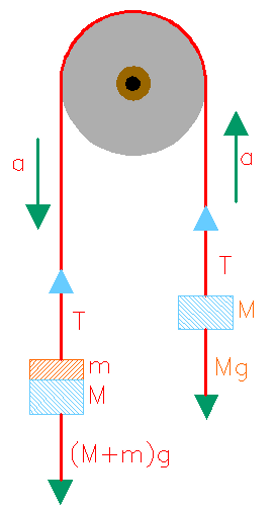
\includegraphics[width=0.25\textwidth]{0650_d1.png}
    \caption{Macchina di Atwood}
    \label{atwoodmachine}
\end{figure}

Dove i corpi hanno massa $m_1,m_2$ rispettivamente e quota $z_1,z_2$ rispettivamente in un riferimento cartesiano centrato nella carrucola (da considerarsi puntiforme) con un asse parallelo al filo e diretto verso il basso. Allora il vincolo della macchina può essere inteso come la lunghezza costante del filo e si può esprimere come segue:
\[f(z)=z_1(t)+z_2(t)-l=0\]
Da cui otteniamo un vincolo per le accelerazioni:
\[\dv[2]{z_1}{t}+\dv[2]{z_2}{t}=0\]
Inoltre per il II principio (posto per comodità $m_2>m_1$ in modo che $a_1<0$):
\[m_1g-|\va{\tau}|=-m_1a_1\quad m_2g-|\va{\tau}|=m_2a_2\]
Otteniamo allora il seguente sistema:
\[\left\{\begin{array}{l}
    a_1(t)+a_2(t)=0  \\
    |\a_1(t)|=a=-g+\frac{|\va{\tau}|}{m_1}\\
    |\a_2(t)|=g-\frac{|\va{\tau}|}{m_2}
\end{array}\right.\]
E quindi l'\textbf{equazione vincolare rispetto alla tensione}:
\begin{equation}
    \boxed{|\va{\tau}|=2g(m_1+m_2)}
\end{equation}
\end{prop}

\begin{prop}
Consideriamo una Macchina composta da due carrucole collegate da un unico filo, una delle quali è mobile ed ha massa non trascurabile, come in figura: 
\begin{figure}[H]
    \centering
    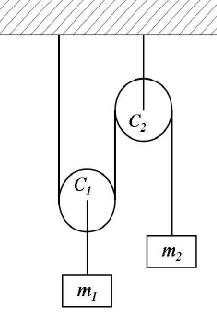
\includegraphics[width=0.25\textwidth]{2i8g76b.png}
    \caption{Carrucola Composta da una mobile e una fissa}
    \label{carrucolamobile}
\end{figure}

Dette $m_1,m_2,m_c$ le masse dei due corpi e della carrucola mobile rispettivamente, allora il vincolo della lunghezza del filo è dato dal sistema:
\[\left\{\begin{array}{l}
    z_2-z_c-l_1=0  \\
    2z_c+z_1-l_2=0 
\end{array}\right.\]
Derivando due volte entrambe le equazioni otteniamo quindi:
\[\left\{\begin{array}{l}
    z_2''(t)-z_c''(t)=0  \\
    2z_c+z_1-l_2=0 
\end{array}\right.\]
\end{prop}


\section{Leggi di Forze}

\subsection{Introduzione}
Tutte forze possono esprimersi come funzioni di $\r,\v,\a,t$ e più in particolare $\r,t$.

\subsection{Forze Notevoli}

\begin{defn}
\textbf{Forza Peso/Forza Gravitazionale}:
\begin{enumerate}
    \item Simbolo: $\va{P}$
    \item Modulo: $m\cdot g$
    \item Direzione: Parallelo al vettore posizione nel sistema di riferimento centrato nel centro della Terra ("verticalre)
    \item Verso: Dal corpo al centro della Terra
    \item Note Ulteriori: \(\va{P}=-G\frac{M_Tm}{r^2}\vu{r}=m\va{g}\)
\end{enumerate}
\end{defn}
\begin{prop}[Legge della Forza di Gravità]
Dati i corpi di masse gravitazionali $m_1,m_2$ e raggi vettori $\r_1,\r_2$ in un certo riferimento allora l'interazione gravitazionale tra il corpo 1 e il corpo 2 è:
\[\f_{12}=G\frac{m_1m_2}{|\r_2-\r_1|^1}\vu{r}_{21}=G\frac{m_1m_2}{|\r_2-\r_1|^2}\frac{(\r_2-\r_1}{|\r_2-\r_1|}=G\frac{m_1m_2}{|\r_2-\r_1|^3}(\r_2-\r_1)=m_1\dv[2]{\r_1}{t}\]
(Per il II Principio).\\
Similmente l'interazione tra il corpo 2 e il corpo 1:
\[\f_{21}=G\frac{m_1m_2}{|\r_1-\r_2|^3}(\r_1-\r_2)=m_2\dv{\r_2}{t}\]
\end{prop}


\begin{defn}
\textbf{Reazione Vincolare Normale}:
\begin{enumerate}
    \item Simbolo: $\va{N}$
    \item Modulo: Dipende dalla condizioni di equilibrio
    \item Direzione: Perpendicolare alla superficie di contatto
    \item Verso: Si oppone alla compenetrazione dei corpi
\end{enumerate}
\end{defn}
\begin{prop}
Quando un punto materiale interagisce con un corpo dalla superficie curva, allora la direzione della forza è sempre perpendicolare alla superficie, stavolta però non è costante.
\end{prop}

\begin{defn}
\textbf{Forza d'Attrito Statica}:
\begin{enumerate}
    \item Simbolo: $\va{f}_a$
    \item Modulo: Dipende dalle condizioni di equilibrio
    \item Direzione: Tangente alla superficie di contatto
    \item Verso: //
\end{enumerate}
\end{defn}
\begin{property}
La Forza d'Attrito Radente si può presentare sotto due regimi:
\begin{enumerate}
    \item \textbf{Regime Statico} in cui la forza d'attrito eguaglia la forza "spingente" e il quale si supera raggiunta una certa forza $\mu_S|\N|$ dove $\mu_S$ è detto \textbf{coefficiente d'attrito statico}.
    \item \textbf{Regime Dinamico} in cui la forza d'attrito ha valore costante $\mu_d|\N|<\mu_S|\N|$ dove $\mu_d$ è detto \textbf{coefficiente d'attrito dinamico}.
\end{enumerate}
Nel caso di un corpo in regime dinamico (ad esempio in discesa lungo un piano inclinato) possiamo determinare le leggi oraria di posizione, velocità e accelerazione a partire dalla risultante delle forze (scelto un sistema di riferimento centrato nella posizione iniziale del corpo, un asse rivolto verso il basso e parallelo al piano, l'altro perpendicolare e uscente):
\[\j) |\N|-mg\cos\alpha=0\iff |\N|=mg\cos\alpha\]
\[\i) mg\sin\alpha-\mu_dmg\cos\alpha=ma\iff a=g(\sin\alpha-\mu_d\cos\alpha)\]
Posto $\lambda^\pm=(\sin\alpha\pm\mu_d\cos\alpha)$ allora le leggi oraria sono le seguenti (con velocità iniziale $v_0$ e istante iniziale $t_0$):
\[\left\{\begin{array}{l}
    x(t)=v_0(t-t_0)-\frac{g\lambda^-}{2}(t-t_0)^2   \\
    v(t)=v_0+g\lambda^-(t-t_0)    \\
    a(t)=g\lambda^-   \\
\end{array}\right.\]
\end{property}



\begin{defn}
\textbf{Tensione di un Filo/Sbarra Ideale}:
\begin{enumerate}
    \item Simbolo: $\va{\tau}$
    \item Modulo: Dipende dalle condizioni di equilibrio
    \item Direzione: Parallela a quella del filo
    \item Verso: Dal corpo al supporto
    \item Note Ulteriori: Un filo ideale si può considerare come un filo composto da infinitesime parti a cui viene applicata una forza dalla precedente e che applicano la stessa forza alla parte successiva, trasmettendo perfettamente la forza dal sostegno al corpo appeso.
\end{enumerate}
\end{defn}


\begin{defn}
\textbf{Forza Elastica}:
\begin{enumerate}
    \item Simbolo: $\va{F}_e$
    \item Modulo: $k\delta l$
    \item Direzione: Parallela all'asse della molla
    \item Verso: Opposto alla deformazione
\end{enumerate}
\end{defn}

\section{Conseguenze dei Principi della Dinamica}

\subsection{Quantità di Moto e Impulso}

\begin{defn}
\textbf{Quantità di Moto} \(\p=m\v\)
\end{defn}
\note \hypertarget{quantità-forza}{Se la massa è costante allora si ottiene}:
\[\dv{\p}{t}=\dv{(m\v)}{t}=m\dv{\v}{t}=m\a=\F\]
Che è una versione più generale del II Principio anche per masse non costanti, tale che possiamo intendere l'interazione di due corpi come una variazione della velocità (in modulo, direzione, verso) oppure la sua massa.

\begin{thm}[Teorema dell'Impulso]
\label{teoremaimpulso}
Detto $\J$ il vettore ottenuto integrando una forza $\F$ applicato in un intervallo di tempo $t$, che chiamiamo \textbf{Impulso della Forza}:
\[\J=\int_0^t\F \dd t\]
Per quanto \hyperlink{quantità-forza}{notato} otteniamo:
\[\J=\int_0^t\F \dd t=\int_0^t\dv{\p}{t} \dd t=\int_{\p_0}^{\p}\dd \p=\p-\p_0=\Delta \p\then \boxed{\J=\Delta\p}\]
Ossia l'applicazione di una forza ad un corpo per un certo intervallo di tempo causa una variazione della quantità di moto.
\end{thm}
\note Se la massa è costante il Teorema dell'Impulso si riduce a:
\[\J=m(\v-v_0)=m\Delta\v\]
Inoltre usando il Teorema della Media Integrale possiamo calcolare il valore medio della forza nota la variazione di quantità di moto:
\[\F_m=\frac{\Delta\p}{t}\]

\begin{prop}[Conservazione della Quantità di Moto]
Diretta conseguenza del Teorema dell'Impulso è che se la risultante delle forze applicate ad un sistema è nulla, allora la quantità di moto si conserva. Per corpi di massa costante tale principio è solo un'estensione del Principio d'Inerzia.
\end{prop}

\subsection{Urti}
\begin{defn}
Un'interazione tra due o più corpi che abbia durata limitata.
\end{defn}

\begin{prop}
Studiare un urto significa misurare le quantità di moto iniziali e finali dei corpi coinvolti. Inoltre, per la Conservazione della Quantità di Moto la variazione totale di quantità di moto è nulla:
\[\Delta\p_1+\Delta\p_2=(\p'_1-\p_1)+(\p'_2-\p_2)=0\]
\end{prop}

\begin{example}
Un esempio di urto tra due corpi può essere anche l'avvicinamento di un asteroide al sole. Tuttavia in una gran parte delle considerazioni relative agli urti si considera che lo spostamento e la durata dell'urto siano entrambe nulle (infinitesime).
\end{example}

\section{Dinamica dei Sistemi}


\end{document}
